% Template for PLoS
% Version 3.6 Aug 2022
%
% % % % % % % % % % % % % % % % % % % % % %
%
% -- IMPORTANT NOTE
%
% This template contains comments intended 
% to minimize problems and delays during our production 
% process. Please follow the template instructions
% whenever possible.
%
% % % % % % % % % % % % % % % % % % % % % % % 
%
% Once your paper is accepted for publication, 
% PLEASE REMOVE ALL TRACKED CHANGES in this file 
% and leave only the final text of your manuscript. 
% PLOS recommends the use of latexdiff to track changes during review, as this will help to maintain a clean tex file.
% Visit https://www.ctan.org/pkg/latexdiff?lang=en for info or contact us at latex@plos.org.
%
%
% There are no restrictions on package use within the LaTeX files except that no packages listed in the template may be deleted.
%
% Please do not include colors or graphics in the text.
%
% The manuscript LaTeX source should be contained within a single file (do not use \input, \externaldocument, or similar commands).
%
% % % % % % % % % % % % % % % % % % % % % % %
%
% -- FIGURES AND TABLES
%
% Please include tables/figure captions directly after the paragraph where they are first cited in the text.
%
% DO NOT INCLUDE GRAPHICS IN YOUR MANUSCRIPT
% - Figures should be uploaded separately from your manuscript file. 
% - Figures generated using LaTeX should be extracted and removed from the PDF before submission. 
% - Figures containing multiple panels/subfigures must be combined into one image file before submission.
% For figure citations, please use "Fig" instead of "Figure".
% See http://journals.plos.org/plosone/s/figures for PLOS figure guidelines.
%
% Tables should be cell-based and may not contain:
% - spacing/line breaks within cells to alter layout or alignment
% - do not nest tabular environments (no tabular environments within tabular environments)
% - no graphics or colored text (cell background color/shading OK)
% See http://journals.plos.org/plosone/s/tables for table guidelines.
%
% For tables that exceed the width of the text column, use the adjustwidth environment as illustrated in the example table in text below.
%
% % % % % % % % % % % % % % % % % % % % % % % %
%
% -- EQUATIONS, MATH SYMBOLS, SUBSCRIPTS, AND SUPERSCRIPTS
%
% IMPORTANT
% Below are a few tips to help format your equations and other special characters according to our specifications. For more tips to help reduce the possibility of formatting errors during conversion, please see our LaTeX guidelines at http://journals.plos.org/plosone/s/latex
%
% For inline equations, please be sure to include all portions of an equation in the math environment.  For example, x$^2$ is incorrect; this should be formatted as $x^2$ (or $\mathrm{x}^2$ if the romanized font is desired).
%
% Do not include text that is not math in the math environment. For example, CO2 should be written as CO\textsubscript{2} instead of CO$_2$.
%
% Please add line breaks to long display equations when possible in order to fit size of the column. 
%
% For inline equations, please do not include punctuation (commas, etc) within the math environment unless this is part of the equation.
%
% When adding superscript or subscripts outside of brackets/braces, please group using {}.  For example, change "[U(D,E,\gamma)]^2" to "{[U(D,E,\gamma)]}^2". 
%
% Do not use \cal for caligraphic font.  Instead, use \mathcal{}
%
% % % % % % % % % % % % % % % % % % % % % % % % 
%
% Please contact latex@plos.org with any questions.
%
% % % % % % % % % % % % % % % % % % % % % % % %

\documentclass[10pt,letterpaper]{article}
\usepackage[top=0.85in,left=2.75in,footskip=0.75in]{geometry}

% amsmath and amssymb packages, useful for mathematical formulas and symbols
\usepackage{amsmath,amssymb}
\usepackage{mathtools}
\usepackage{amsthm}

% Use adjustwidth environment to exceed column width (see example table in text)
\usepackage{changepage}

% textcomp package and marvosym package for additional characters
\usepackage{textcomp,marvosym}

% cite package, to clean up citations in the main text. Do not remove.
\usepackage{cite}

% Use nameref to cite supporting information files (see Supporting Information section for more info)
\usepackage{nameref,hyperref}

% line numbers
\usepackage[right]{lineno}

% ligatures disabled
\usepackage[nopatch=eqnum]{microtype}
\DisableLigatures[f]{encoding = *, family = * }

% color can be used to apply background shading to table cells only
\usepackage[table]{xcolor}

% array package and thick rules for tables
\usepackage{array}

\usepackage{pslatex}
%\usepackage{apacite}

\usepackage{cancel}
% The color of hyperlinks (URLs)
%\usepackage[backend=bibtex,style=nature,natbib=true]{biblatex} 
%\usepackage{biblatex} 
%\usepackage{natbib}


% create "+" rule type for thick vertical lines
\newcolumntype{+}{!{\vrule width 2pt}}

% create \thickcline for thick horizontal lines of variable length
\newlength\savedwidth
\newcommand\thickcline[1]{%
  \noalign{\global\savedwidth\arrayrulewidth\global\arrayrulewidth 2pt}%
  \cline{#1}%
  \noalign{\vskip\arrayrulewidth}%
  \noalign{\global\arrayrulewidth\savedwidth}%
}

% \thickhline command for thick horizontal lines that span the table
\newcommand\thickhline{\noalign{\global\savedwidth\arrayrulewidth\global\arrayrulewidth 2pt}%
\hline
\noalign{\global\arrayrulewidth\savedwidth}}


% Remove comment for double spacing
%\usepackage{setspace} 
%\doublespacing

% Text layout
\raggedright
\setlength{\parindent}{0.5cm}
\textwidth 5.25in 
\textheight 8.75in

% Bold the 'Figure #' in the caption and separate it from the title/caption with a period
% Captions will be left justified
\usepackage[aboveskip=1pt,labelfont=bf,labelsep=period,justification=raggedright,singlelinecheck=off]{caption}
\renewcommand{\figurename}{Fig}

% Use the PLoS provided BiBTeX style
%\bibliographystyle{plos2015}

% Remove brackets from numbering in List of References
%\makeatletter
%\renewcommand{\@biblabel}[1]{\quad#1.}
%\makeatother



% Header and Footer with logo
\usepackage{lastpage,fancyhdr,graphicx}
\usepackage{epstopdf}
%\pagestyle{myheadings}
\pagestyle{fancy}
\fancyhf{}
%\setlength{\headheight}{27.023pt}
%\lhead{\includegraphics[width=2.0in]{PLOS-submission.eps}}
\rfoot{\thepage/\pageref{LastPage}}
\renewcommand{\headrulewidth}{0pt}
\renewcommand{\footrule}{\hrule height 2pt \vspace{2mm}}
\fancyheadoffset[L]{2.25in}
\fancyfootoffset[L]{2.25in}
\lfoot{\today}

%% Include all macros below

\newcommand{\lorem}{{\bf LOREM}}
\newcommand{\ipsum}{{\bf IPSUM}}

%% END MACROS SECTION

% Some field suppression via options
\ExecuteBibliographyOptions{isbn=false,url=false,doi=false,eprint=false}

% One-paragraph bibliography environment
\defbibenvironment{bibliography}
  {\list
     {\printtext[labelnumberwidth]{%
        \printfield{prefixnumber}%
        \printfield{labelnumber}}%
      \ifentrytype{article}{% Suppress remaining fields/names/lists here
        \clearfield{title}}{}}
     {\setlength{\leftmargin}{0pt}%
      \setlength{\topsep}{0pt}}%
      \renewcommand*{\makelabel}[1]{##1}}
  {\endlist}
  {\mkbibitem}

% \mkbibitem just prints item label and non-breakable space
\makeatletter
\newcommand{\mkbibitem}{\@itemlabel\addnbspace}
\makeatother

% Add breakable space between bibliography items
\renewcommand*{\finentrypunct}{\addperiod\space}

% et al. string upright (nature style applies \mkbibemph)
\renewbibmacro*{name:andothers}{%
  \ifboolexpr{
    test {\ifnumequal{\value{listcount}}{\value{liststop}}}
    and
    test \ifmorenames
  }
    {\ifnumgreater{\value{liststop}}{1}{\finalandcomma}{}%
     \andothersdelim
     \bibstring{andothers}}
    {}}

\addbibresource{biblio.bib} % The filename of the bibliography
\usepackage{color}




\begin{document}
\vspace*{0.2in}

% Title must be 250 characters or less.
\begin{flushleft}
{\Large
\textbf\newline{Balancing accuracy and diversity : principles of model-driven active sampling in the brain} % Please use "sentence case" for title and headings (capitalize only the first word in a title (or heading), the first word in a subtitle (or subheading), and any proper nouns).
}
\newline
% Insert author names, affiliations and corresponding author email (do not include titles, positions, or degrees).
\\
Name1 Surname\textsuperscript{1,2\Yinyang},
Name2 Surname\textsuperscript{2\Yinyang},
Name3 Surname\textsuperscript{2,3\textcurrency},
Name4 Surname\textsuperscript{2},
Name5 Surname\textsuperscript{2\ddag},
Name6 Surname\textsuperscript{2\ddag},
Name7 Surname\textsuperscript{1,2,3*},
with the Lorem Ipsum Consortium\textsuperscript{\textpilcrow}
\\
\bigskip
\textbf{1} Affiliation Dept/Program/Center, Institution Name, City, State, Country
\\
\textbf{2} Affiliation Dept/Program/Center, Institution Name, City, State, Country
\\
\textbf{3} Affiliation Dept/Program/Center, Institution Name, City, State, Country
\\
\bigskip

% \author{\large \bf Anonymous authors}
%\author{{\large \bf Hamza Oueld (hamza.oueld-kaddour-el-hallaloui@univ-amu.fr)}$^{1}$ \\
%\AND {\large \bf Andrea Brovelli (andrea.brovelli@univ-amu.fr)}$^{1}$ \\
%\AND {\large \bf Emmanuel Daucé (emmanuel.dauce@univ-amu.fr)}$^{1,2}$ \\
%1.Institut de Neurosciences de la Timone, Aix-Marseille Univerity, 
%Marseille, France\\
%2.Ecole Centrale de Marseille,
%Marseille, France
%}

% Insert additional author notes using the symbols described below. Insert symbol callouts after author names as necessary.
% 
% Remove or comment out the author notes below if they aren't used.
%
% Primary Equal Contribution Note
\Yinyang These authors contributed equally to this work.

% Additional Equal Contribution Note
% Also use this double-dagger symbol for special authorship notes, such as senior authorship.
\ddag These authors also contributed equally to this work.

% Current address notes
\textcurrency Current Address: Dept/Program/Center, Institution Name, City, State, Country % change symbol to "\textcurrency a" if more than one current address note
% \textcurrency b Insert second current address 
% \textcurrency c Insert third current address

% Deceased author note
\dag Deceased

% Group/Consortium Author Note
\textpilcrow Membership list can be found in the Acknowledgments section.

% Use the asterisk to denote corresponding authorship and provide email address in note below.
* correspondingauthor@institute.edu

\end{flushleft}
% Please keep the abstract below 300 words
\section*{Abstract}
Understanding our environment requires not only passively observing sensory samples but also \emph{acting} to seek out useful relationships between our actions and their possible outcomes. Inspired by the principle of visual salience, we introduce the concept of an "ideal participant", which is the active counterpart of a Bayesian ideal observer. During learning, an ideal participant would build a statistical model of its environment while updating its policy (action selection) after each new observation. This action selection requires a tight balance between making correct predictions (accuracy) and providing diverse data to feed the models (diversity).
We assess these principles in a knowledge-oriented action selection task called the "volleyball" task, where participants estimate the causal influence of a player on the outcome of a volleyball game. The behavioral data we have collected suggest that such active sampling strategies do occur in the brain and improve the accuracy of action/outcome models. We show that the balance between accuracy and diversity objectives can lead to specific action selection biases, reflected both in the model and in the experiments.

% Please keep the Author Summary between 150 and 200 words
% Use first person. PLOS ONE authors please skip this step. 
% Author Summary not valid for PLOS ONE submissions.   
\section*{Author summary}

{\color{gray}
%The hypothesis that actions serve to sample sensory data posits that body movements are sources of sensory changes, facilitating active learning by enhancing data inference. According to this view, actions are not merely responses to external stimuli but are proactive processes aimed at gathering information about the environment. By actively engaging with their surroundings, organisms can improve their understanding and predictions of environmental states \citep{clark2013whatever}.
Active learning suggests that the purpose of actions is to minimize uncertainty by continuously updating internal models based on new sensory inputs. This process is akin to hypothesis testing, where the brain generates predictions and then tests these predictions against actual sensory data. %Such an approach allows the brain to refine its models, making them more accurate and reliable over time. % \citep{sutton2018reinforcement}.
%The concept of active inference further elaborates on this hypothesis by proposing that actions are aimed at minimizing posterior prediction error. This is achieved through the maximization of novelty or Bayesian surprise, where the brain seeks out new and unexpected sensory data to reduce uncertainty in its predictive models. By continually seeking out novel experiences, the brain can challenge and update its models, ensuring they remain relevant and effective \citep{friston2010action}.
%This framework suggests that the brain operates in a constant loop of prediction and correction, where prediction errors signal the need for model adjustment. The minimization of prediction error through active inference is a core principle of this model, relying on the Bayesian framework to update beliefs and predictions \citep{rao1999predictive}. This dynamic interaction with the environment is essential for maintaining a high level of adaptability and for optimizing behavior in a constantly changing world \citep{friston2015active}.
The hypothesis that actions serve to sample sensory data underscores the importance of proactive engagement with the environment in sensory perception and cognitive function. 
%Through active learning and the minimization of prediction errors, organisms can refine their internal models, better anticipate changes in their surroundings, and enhance their overall adaptability and survival.
}

\linenumbers


%    Significance

%commencer par le paradoxe des pigeons qui choisissent une action de manière aleatoire (+ aller voir les refs Boraud). 
%Le comportement consiste alors a biaiser les reponses vers une réponse particulière, velle qui apporte le meilleur rendement. Néanmoins, la strategie suivie par ls animaux est souvent loin de la stratégie optimale (thompson sampling).

%Une hypothèse a été émise comme quoi le cerveau construit des descriptions probabilistes des relations entre ses actions et les effets de ses actions. model-based vs model free action selection.  
%A striking property of the brain is its natural capability to infer statistical relationships between the observed variables of its environment, through a large variety of experimental setups [refs]. 

\section{Introduction}

Information-seeking behavior is a fundamental aspect of both human and animal cognition, driven by the need to reduce uncertainty and enhance understanding of the environment. This behavior primarily involves anticipating the informational content that a movement, action, or sensor shift will provide, and making choices based on the maximization of this expected information. This model-based action selection relies on the presence of a predictive model that enables the anticipation of the consequences of actions \cite{friston2010free}.

The presence of such a model allows for the measurement of deviations from predictions, a concept central to predictive coding \cite{rao1999predictive}. Predictive coding posits that the brain continuously generates predictions about sensory inputs and then adjusts these predictions based on the actual input received. The discrepancies, or prediction errors, between expected and actual inputs are central for several cognitive processes, including visual perception and efficient coding \cite{rao1999predictive,ITTI20091295}, novelty and change detection \cite{behrens2007learning, summerfield2009expectation,garrido2013outlier}, exploration/exploitation trade-off \cite{cohen2007should,wilson2014humans}, and learning \cite{schulz2007serious,oudeyer2016intrinsic}.

Crucially, information-seeking behavior is not just about reacting to prediction errors but involves the anticipation of these errors. This means that individuals engage in actions that they expect will maximize future prediction errors, thereby maximizing the informational gain. This anticipation of prediction errors, or the expected surprise, drives exploratory behavior and guides the search for new information \cite{friston2012perceptions}.
Research on decision-making and information-seeking has provided robust theoretical frameworks for understanding this anticipatory aspect of information-seeking. Oaksford and Chater \cite{oaksford1994rational} demonstrated that human participants select information in a manner that maximizes the \emph{expected information gain} (EIG), rather than random exploration, reflecting a rational approach to data selection based on Bayesian principles. Similarly, Nelson \cite{nelson2005finding} developed a Bayesian framework to explain curiosity-driven behavior, showing that individuals seek information to maximize the reduction of uncertainty. Similar principles are moreover suggested to take place in animal behavior \cite{gottlieb2013information,kidd2015psychology}.

From the machine learning perspective, information-seeking is crucial in reinforcement learning (RL) and active learning, primarily addressing the exploration-exploitation dilemma. In multi-armed bandit problems, strategies such as Thompson Sampling and EXP3 effectively balance exploration and exploitation to maximize reward and gather new information \cite{robbins1952some, sutton1988learning, thompson1933likelihood, chapelle2011empirical, auer2002finite}. However, in more complex temporal credit assignment problems, where decisions impact future rewards across multiple steps, exploration often relies on random choices or heuristics \cite{sutton1998introduction}. To enhance exploration, methods such as pseudo-counts and expected information gain have however been proposed, where pseudo-counts estimate the novelty of states or actions, guiding exploration towards less familiar areas \cite{bellemare2016unifying}, while expected information gain integrates the potential for new information into the reward function, encouraging actions that maximize knowledge acquisition [REFS].

{\color{blue}
\emph{Salience and information in the brain.}
[TODO]
La réduction de l'incertitude apparait comme un des principes fondamentaux grace auxquels le cerveau intègre et synthétise les informations en provenance de l'environnement, incluant à la fois la formation à long terme des champs récepteurs de neurones dans le cas du codage prédictif [ref], mais également l'intégration d'indices sensoriels multiples dans la résolution d'ambiguités perceptives [ref]. %La perception de l'écart entre le signal attendu et le signal effectif est un marqueur fondamental de 
Il est ainsi reconnu de longue date que la mesure de l'écart à la distribution attendue est sous-jacent à de nombreux processus cognitifs et inférentiels [REF], implpiquant le cortex XX et de nombreuses aires XX.
Par ailleurs, un aspect classique de la prise de décision dans un contexte d'incertitude concerne bien sûr la mesure du risque empirique et les choix liés à la réduction de ce risque en vue de maximiser un bénéfice, mettant en oeuvre le réseau de la prise de décision XXX implicant les aires XXX.

Néanmoins, en l'absence de bénéfice ou de coût évident (extérieur), %nécessitent également la prise en compte de l'incertitude dans le choix de l'action, 
le rôle de la perception (ou de la prédiction) de l'incertitude dans la sélection de l'action est moins bien connu et moins bien documenté. [A DEVELOPPER]}


%Neuroscientific research has indicated that various brain regions, including the prefrontal cortex, anterior cingulate cortex, and the insula, are involved in encoding uncertainty. For instance, the prefrontal cortex is thought to integrate sensory information and contextual clues to form probabilistic representations of the environment \cite{doya2007bayesian}. The anterior cingulate cortex has been implicated in conflict monitoring and decision-making under uncertainty, reflecting the brain's effort to resolve discrepancies between expected and actual outcomes \cite{botvinick2004conflict}. Additionally, the insula is associated with the subjective experience of uncertainty and risk, processing the emotional responses related to uncertain situations \cite{paulus2006insular}. Understanding these neural mechanisms is essential for developing models that accurately reflect how uncertainty influences cognitive processes and behavior.
% József Fiser and colleagues have explored how the brain employs Bayesian inference to represent and manage uncertainty, suggesting that neural circuits are optimized to predict sensory inputs in a probabilistic manner \cite{fiser2010statistically}. Máté Lengyel's work has highlighted the role of synaptic plasticity in learning probabilistic representations, demonstrating how neural networks can adapt to uncertain environments \cite{lengyel2015hippocampal}. Florent Meyniel has contributed to the field by investigating how the brain tracks the volatility of the environment, proposing that the brain continuously updates its beliefs based on the reliability of incoming information \cite{meyniel2016human}. These studies underscore the complexity and sophistication of neural mechanisms underlying the representation of uncertainty.

%



The aim of this article is to revisit information-seeking behavior in the case where subjects receive instructions to evaluate the causal link between their actions (interventions) and the resulting outcomes, without maximizing the total outcome. In this context, the problem reduces to assessing whether actions have an effect on the outcomes, and whether this effect is positive or negative at the final result level. The setup makes it possible to compare the subjects' behaviors with different action-selection models to determine the extent to which behavior arbitrates between information selection, random choice, and the pursuit of positive outcomes. Because estimating expected information gains is computationally expensive, we specifically seek to estimate how human behavior deviates from the expected optimal behavior (named here the ``ideal participant'') and reflects strategic choices involving a trade-off between the cognitive load of anticipation and the accuracy of the response.

In particular, we develop a method combining (exact) sequential bayesian inference with Thompson sampling for model comparison and causal inference. The key concepts manipulated are the concept of \emph{expected improvement} and   
\emph{information seeking}, in relation with the problem of sequential design.

% en particulier : 
% - nous proposons une redéfinition de bayesian surprise en lien avec bayes factor/bayes ratio??
% - utilisation de thompson sampling dasn un cadre ou on ne cherche pas a maximiser reward --> nouveau?? --> lien avec estim de l'EIG via MCMC??  --> les échantillons qui représentent l'incertitude des paramètres.

\section{Problem setting}

Our environment is full of unpredictable events, and the Bayesian brain hypothesis \cite{knill2004bayesian} suggests that our brains build models to better predict these events. This assumption relies on the idea that the sensory environment acts as a source of random events, against which the brain would construct probabilistic models that would enable it to better predict and anticipate these events \cite{friston2005theory}. This is also known as inference, in the sense that the brain would start from a certain number of hypotheses about the state of the environment, and use the available data to confirm or eliminate some of them. A fundamental feature of this inference process is its predictive nature, which means that the brain's predictions can be compared with the actual data \cite{rao1999predictive}. It is generally assumed that these predictions are obtained by sampling the probabilistic model, and that the validity of the model (or of the hypotheses) is compared with the accuracy of the predictions made \cite{griffiths2008bayesian}. The framework of model inference is considered as a plausible mechanism of learning in the brain, where updating the model according to the prediction error is the central operation, based on Bayes' rule \cite{doya2007bayesian,fiser2010statistically}.

%Crucially, at no point does it "see" probabilities; it only sees realizations. 
%This is referred to as (Bayesian) inference. 

From the formal standpoint, learning the statistical structure of the environment is a typical estimation problem \cite{bishop2006pattern}. Its numeric implementation implies doing some prior assumptions on the statistical model to use, and then estimating its parameters under the Bayesian framework from observing samples \cite{gelman1995bayesian}. The parameters of the model play here the role of a hidden variable, that are \emph{inferred} from observing their outcome. In that framework, a typical objective is the maximization of the likelihood of the outcome, given the parameters (Maximum Likelihood Estimate) \cite{myung2003tutorial}, or the maximization of the Evidence Lower Bound (ELBO), a compound objective also considering minimizing the complexity of the model \cite{kingma2013auto,blei2017variational}.

This probabilistic approach has long been used as a plausible mechanism of visual perception, where the statistical distribution of natural images, under the constraint of parsimony, allows to explain the formation of orientation receptive fields in V1 \cite{simoncelli2001natural}, as well as certain "extra-classical" receptive fields \cite{rao1999predictive}. The visual system seems to operate similarly to an "ideal" Bayesian estimator \cite{geisler1989sequential,geisler2008visual}. It is also interesting to note that the same fundamental principles of estimating a latent distribution from a large number of examples is at the core of unsupervised learning, e.g. in variational auto-encoders and image generation \cite{hinton1995wake, kingma2013auto, rombach2022high}.


%Cependant, ce principe d'estimation ne semble pas se cantonner au simple système visuel et apparaît comme un mécanisme très général grâce auquel le cerveau adapte de manière flexible ses choix et ses réponses aux données de l'environnement \cite{friston2010free}. Si l'estimation de données et la prédiction semblent constituer le mécanisme à travers lequel sont traitées les données sensorielles \cite{knill2004bayesian}, il semble, de manière plus fondamentale, que ce même principe pourrait également s'appliquer à la sélection de l'action . Il existe en effet une correspondance classique entre la sélection de l'action et l'estimation, en particulier dans le cadre du contrôle optimal basé sur les modèles, pour lesquels le modèle de la commande s'appuie sur le modèle de l'environnement \cite{}.

However, this principle of estimation through a generative model does not seem to be confined to the visual system alone and appears as a general mechanism by which the brain flexibly adapts its choices and responses to environmental data . If model estimation and prediction seem to constitute the mechanism through which sensory data is processed, it seems, in a more fundamental way, that this same principle could also be applied to action selection \cite{friston2010free}. 

\begin{itemize}
\item On the one side, there is a classic correspondence between action selection and estimation, particularly in the context of model-based optimal control, where the control model rests on inverting the (forward) model of the environment \cite{todorov2001optimal,kording2004bayesian}, on contrary to the model-free context, where learning the policy rests on selecting an action that will maximize the cumulative sum of rewards \cite{sutton1998introduction}. %which, in the simple bandit case, resumes to maximizing the outcome itself 
Even in that last case however, a statistical Bayesian framework may also conduct to consider the policy as a parametric \emph{probability on action}, with maximizing the outcome interpreted as maximizing the (log)-likelihood of the policy (in a policy parametric space) [Levine]. %Put in such a probabilistic framework, action selection becomes a part of a more general 
%Then, predictive coding \cite{rao1999predictive} reflects the capacity of sampling those probabilities to predict what we'll sense. 
\item On the other side, as our body's movements affect what we sense, the active inference framework assumes that we  learn by making purposeful moves to understand our surroundings better \cite{friston2012perceptions} . %We choose our actions based on estimating information or prediction errors. 
Interestingly, in that framework, the goal is not only to minimize errors in our predictions, but also maximizing novelty or surprise, in order to seek out information, a concept known as Bayesian surprise \cite{ITTI20091295}. Maximizing novelty  is indeed important if one expect to better understand one's environment and avoid future misinterpretations. This search of novelty %as an interpretation of movement selection 
was first proposed by Itti and Baldi \cite{ITTI20091295}, telling that the eye is attracted by the part of the visual scene that is the most surprising regarding the current data model (i.e. the current interpretation). Put in a Bayesian framework, this corresponds to maximizing model update, given the available data, measured here as a Kullback-Leibler divergence between the old and the new models, seen as a proxy for the prediction error \emph{reduction} after observing new data. This quantification of novelty appeared later on to have a pivotal role in the theory of active inference, where it is referred as the ``epistemic value'' of sensory data [REF]. Say in short, one should put attention to the interpretation errors that significantly contribute to minimizing future prediction errors. 

%[LINK WITH INFORMATION THEORY]
% Tishby and Polani introduced the concept of empowerment within the framework of information theory as a measure of an agent's ability to influence its future state through its actions. Empowerment is quantified by the channel capacity between an agent's current actions and its future states, effectively measuring the entropy of the future states that the agent can achieve \cite{tishby2011information, polani2006formal}. This concept is closely related to the information bottleneck principle, which aims to find a compressed representation of an input variable that preserves the most relevant information about an output variable \cite{tishby2000information}. In the context of empowerment, the goal is to maximize the mutual information between actions and future states, akin to maximizing relevant information in the information bottleneck framework. By maximizing empowerment, an agent adopts behaviors that enhance its control and adaptability, making it more robust and flexible in dynamic environments \cite{klyubin2005empowerment}. These ideas have significant implications for developing autonomous systems in robotics and artificial intelligence, providing a theoretical basis for adaptive and resilient behavior.

%This principle can be generalized by assuming that our sensory environment

In complement, the magnitude of the actual prediction error made by the model, in other words the "surprise", is related to the concept of entropy and information: data is more informative the more it deviates from the expected distribution. In a sensorimotor context, Tishby and Polani have shown that an agent has the capability to control information by maximizing the entropy of the distribution of observed states through its actions \cite{Klyubin2005EmpowermentAU}. More precisely, they introduce the concept of ``Empowerment'', which refers to the capacity of the ``communication channel'' between the agent's actions and the observed states.
In the context of Empowerment, the goal is to maximize the mutual information between actions and future states, akin to maximizing relevant information in the information bottleneck framework \cite{tishby2000information}.
\end{itemize}





Importantly, the two principal objectives, i.e. either reaching nominal response or maximizing information, are not necessarily compliant, which is reminiscent of the  "exploration/exploitation trade-off", at the core of reinforcement learning \cite{sutton1998introduction}. However, quite surprisingly, no satisfactory solution has emerged to date to conciliate model learning (through information seeking) with optimal policy learning.
%[les developpements mathématiques de ces idées conduisent à une situation plutot confuse où de nombreux modèles concurrents de surprise sont employés, souvent dans le cadre de l'optimisation motrice / sélection de l'action, sans qu'il soit évident de les départager. La démarche adoptée dans cet article consiste à analyser dans le détail une situation de choix d'action motivée par l'apprentissage d'une relation de cause à effet entre les actions choisies par le sujet et les effets attendus. Il ne s'agit pas ici de maximiser une récompense future, mais plutot de développer la connaissance la plus précise possible du lien entre les choix faits et leurs conséquences observables, en présence de bruit. Dans ce cadre extrêmement simplifié, nous verrons que l'utilisation d'un modèle hiérarchique permet de rendre compte des principales quantités d'intérêt à l'oeuvre dans les modèles de sélection de l'action, et de les comparer, en tant que modèles de décision, aux choix réellement effectués par des sujets humain. En particulier, l'utilisation  de données electrophysiologiques (MEG) permettent de mettre en évidence les réseaux cérébraux à l'oeuvre dans la prise en compte de ces différentes quantités.]
More detrimentally, the developments of these ideas lead to a rather confusing situation where many competing models of surprise are employed (i.e. Bayesian surprise, Variational Free Energy, Empowerment, Pseudo-count \cite{bellemare2016unifying}, Learning Improvement \cite{schmidhuber1991curious} etc.), either through motor optimization, action selection or in decision making, without it being obvious how to differentiate between them. Ironically, list of about 18 possible surprise definitions (!) was proposed recently \cite{modirshanechi2022taxonomy}. 

The approach adopted in this article involves a detailed analysis of a minimal estimation problem where the agent is motivated by providing an accurate estimate of action outcomes rather than maximizing the expected outcomes, in the presence of noise.  %. This is not about maximizing future rewards but rather about developing the most precise knowledge possible of the link between choices made and their observable consequences
We show that, framed as a hierarchical Bayesian model estimation problem, the concepts of that accounts for the main quantities of interest in action selection, allowing  for comparison with the actual choices made by human subjects. In particular, the use of electrophysiological data (MEG) highlights the brain networks involved in considering these different quantities. %\cite{brookes2011measuring}.

%It was proposed by Itti and Baldi  that the eye is attracted by the part of the visual scene that is the most surprising regarding the (sensory) data model. 
%This principle can be generalized by assuming that our sensory environment
%is mostly interpreted through acting (first) and (then) observing the sensory consequences of our actions. 
%This model-oriented action selection principle is consistent with a Bayesian observer that requires more data to construct his model. 
%More recently, it was proposed by  that the brain may act as a scientific investigator, that would select an action so as to validate (or dismiss) a current hypothesis about the state of the environment.  
%In that case, the difference between the model predictions and the actual sensory observations serves as a metric to interpret the current observation as more or less surprising, 
%and adapt either the model or the action selection so as to minimize the global surprise (that is the surprise over both past and future observations).

%    Originality

%Taking inspiration from Itti and Baldi saliency principle, the idea here is to select actions in a way that should maximize the knowledge about the data model. Let $\pi$ be the \emph{policy}, i.e. an adaptive action selection strategy, and let $\theta$ be the parameters of a data model, that reflects the distribution of expected sensory observations and outcomes observed after an action $a$. Let  $s \in \mathcal{S}$ be the state observed after an action $a$ is actuated.
%Then $p(O|a, \theta)$ is a parametric model of state transitions, that describes the expected distribution of outcomes given an action and the parameters. In a Bayesian setup, $\theta$ is interpreted as a latent variable that explains the current observation. Then, let $q(\theta)$ be a distribution over the latent parameters (posterior distribution) that is updated after each observation. In the simplest case, $p$ is a Bernouilli distribution and $q$ is a beta model over the the (single) parameter of $p$. 

% In model-based reinforcement learning, the statistical relationships between the actions and their outcomes inform the policy for the choice of the action. These statistical relationships can be given in advance, or learned from experiencing action/outcome samples. In the last case, the choice of action (policy) reflects a balance to be kept between two concurrent objectives, one objective being the building of an accurate model of the world, the second one being the maximization of the (cumulative) rewards. The difficulty in balancing exploration and exploitation, in the absence of a definite model, is at the heart of reinforcement learning problems. 

% NOTE : les choix d'actions basés sur la minimisation de la MLE conduisent à des actions stéréotypées. A l'inverse, les comportements baséss ur la maximisation de la surprise conduisent à une "attirance pour le bruit".

% NOTE : qu'est-ce qui doit être perçu pour accéder à l'informaton? différence de deux entropies? expected information gain?
{\color{magenta} Problème : le gain d'information peut-il etre estimé et anticipé?}

% en statistiques : Lindley (1956) : On a measure of the information provided by an experiment? 

% The expected information gain principle (EIG) explained in Smith, F. B., Kirsch, A., Farquhar, S., Gal, Y., Foster, A., & Rainforth, T. (2023, April). Prediction-oriented bayesian active learning.

% en comportement animal/humain : Berlyne, D. E. (1966) : L'une des premières études sur la curiosité et la recherche d'informations, examinant comment la curiosité motive les individus à chercher activement des informations. Référence : Berlyne, D. E. (1966). Curiosity and exploration. Science, 153(3731), 25-33. --> notion de "dissonnance conitive" et de surprise. 

%On the other sie, l }

\section{Experiments }

{\color{blue} The Causal project [TODO] 
\begin{itemize}
    \item sequential estimation
    \item model comparison
    \item causal score, DP, literature
\end{itemize}
}
\subsection{The ``Volleyball'' task}
We consider here a simple model estimation task, where a conditional distribution $p(O|A)$ %(where the outcome $o \in O$ conditionally depends on the action $a \in A$). 
has to be guessed from observing samples. %We want to understand whether the behavior adopted in information-seeking situations resembles that of saliency-based saccade selection in vision, i.e. if action selection is oriented toward the actions whose statistics differs the most from the average outcome statistics, that is the one that maximises the ``Bayesian surprise'' or ``Epistemic Value''. To this end, we consider here a minimal estimation problem consisting of estimating the expected outcome of two concurrent Bernouilli distributions. 


We consider in the following behavioral task called the "Volleyball" task (see figure \ref{fig:1})\cite{basanisi2021neurophysiological}, in which participants are asked to estimate the causal influence of a particular player in making the volley-ball team win or lose the matches. 15 different scenarios are considered. Each scenario is described by two Bernoulli distributions : $p_1=p(o=\text{WIN}|a=\text{PLAY})$ and  $p_0=p(o=\text{WIN}|a=\text{NOT PLAY})$ that reflect the probability to win when the player is selected versus non selected. The influence of the player is thus quantified by the probability difference $\Delta p = p_1 - p_0$, that is a classical measure of action-outcome causality in experimental psychology [REFS]. In a first series of experiments (``setting A''), that difference can vary from strong worsening ($\Delta p = -0.6$ winning probability) to strong improvement ($\Delta p = 0.6$ winning probability). In a second series of experiments (``Setting B''), the influence of the player can only vary from neutral (no change) to strong improvement ($+0.8$ winning probability).
By alternating 'PLAY' and 'NOT PLAY', the human participants obtains samples of 'WIN' and 'LOSE' and are expected to estimate both distributions (which is asked after 40 trials).

\begin{figure}[h]
\centering
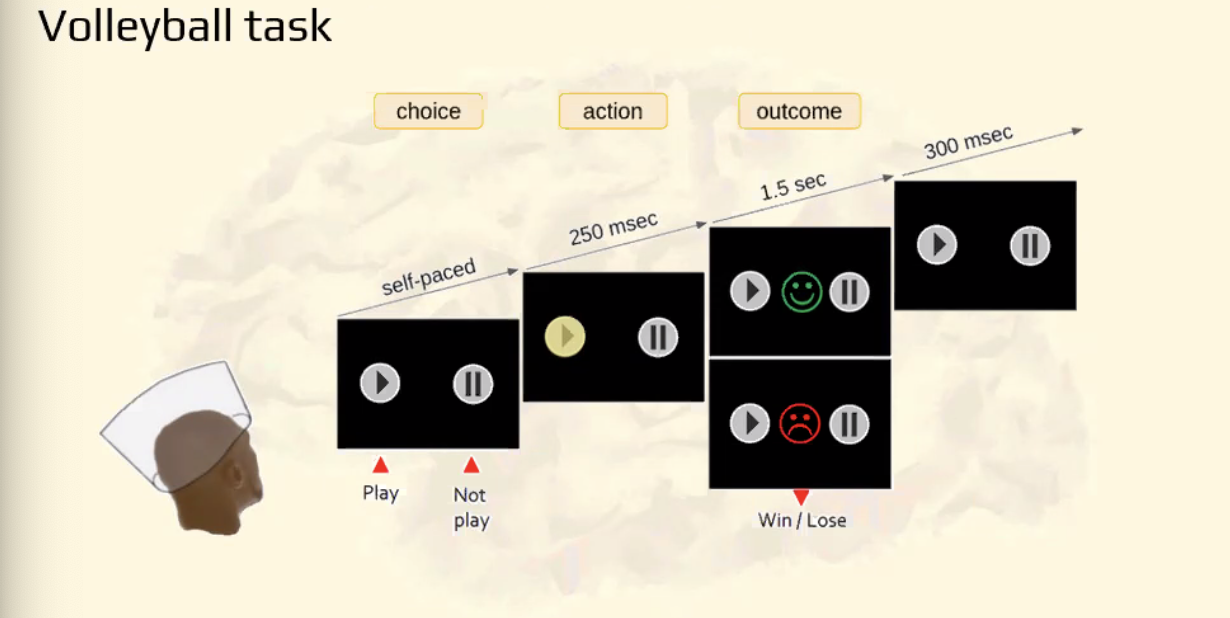
\includegraphics[width=\textwidth]{figs/vb_task.png}
\caption{Participants in the "Volleyball" task act as trainers tasked with hiring players for different teams. They can simulate the outcome of 40 matches with or without a particular player. They have to decide before each match whether to include the player or not ("PLAY" or "NOT PLAY"). Then, they observe the match outcome, and repeat the process until all 40 trials are completed. They are finally asked to assess the player effect on the team's performance.}
\label{fig:1}
\end{figure}

This task addresses the question of action selection when the main objective is to learn a model of the action-outcome relationship, in order to make an appropriate ``buy'' decision. In that case, the participant needs to make a series of actions (PLAY/NOT PLAY) under an objective that is estimate the statistical relationship between actions and outcomes, i.e. the effect of the new player on the team statistics.

\subsection{MEG experiment}
{\color{blue}  [TODO] }
\subsection{SEEG experiment}
{\color{blue}  [TODO] }


\section{Intervention through action: the brain as an ideal sampler}

%We propose in this paper to extend this principle toward the case of model building in goal-directed action selection tasks: what is the appropriate strategy to choose when the objective is to understand the relationship between different actions and an their outcomes? 
In order to compare with subject's decisions, we conceptualize an agent having to take decisions in a stochastic environment where the result of the action (outcome) is uncertain.
We assume that the agent has to learn the effect of its action by interacting with the environment. During learning, the agent will do two things : (i) build a statistical model of its environment and (ii) update its behavior (selection of actions). 


%I
Notations :
\begin{itemize}
    \item $a \in \mathcal{A}$ : action (decision or motor command)
    \item $o \in \mathcal{O}$ : outcome : state observed after action $a$ is actuated
    %\item $r \in \mathbb{R}$ : (quantitative) reward 
    %\item $Q(a)$ : action-value function = policy parameters
    %\item $\pi(a|Q)$ : (stochastic) action selection = policy
    \item $\theta$ : statistic model parameters %(mean, variance)
    \item $p(o|a)$ : (unknown) action/outcome statistical relationship
    \item $q(\theta|o_{1:t},a_{1:t})$ : (posterior) distribution of model parameters. In practice : $\beta$-model 
\end{itemize}





\subsection{Beta ideal observer}


%Both the model and the policy are parametric models. 

%A typical strategy is trying different actions, observing their outcomes and memorizing the average outcome for each action.  

The first element we need to consider is thus describing a mechanism of model estimation. The Bayesian estimation framework allows to formalize the principles of an ``ideal observer''.
Importantly, by construction, an observer does not intervene onto the data it observes. It is a pure passive method of estimation.    

%Let us start with a more formal description of the estimation problem at stake.
A Bayesian ideal observer \cite{geisler1989sequential} experiments the statistical structure of its environment from observing a series of samples, without intervening on it. It generally assumes a parametric model $\theta$ to explain the observations $o_1, o_2, ...$, with each $o_t$ assumed a sample of $p(O|\theta)$, $\theta$ being unknown. At every step of the process, the agent forms an estimate of the parameters, $q(\Theta|h_{t-1}, o_t)$ with $h_{t-1}$ the sequence of past observations and $o_t$ the current observation. Then, the update of the model rests on applying Bayes formula on the new data using the chain rule: $q(\Theta|h_{t-1}, o_t) \propto p(o_t|\Theta) q(\Theta|h_{t-2}, o_{t-1})$.

In the case of a Bernoulli series of observations $o_1,...,o_t$, the update of a Beta model [REF] can be shown to follow that of a Bayesian ideal observer. 
\begin{equation}
    \theta_t \sim \text{Beta}(\alpha_t,\beta_t)
\end{equation}
with $\alpha_0$ = $\beta_0$ = 1 and for $t>0$:
\begin{equation}
    (\alpha_t,\beta_t) = \left\{
    \begin{array}{ll}
        (\alpha_{t-1}+1,\beta_{t-1}) & \mbox{if $o_t=\text{WIN}$} \\
        (\alpha_{t-1},\beta_{t-1}+1) & \mbox{otherwise}. \\
    \end{array}
\right.
\end{equation}

Consider now a series of actions and outcomes, instead of outcomes alone. 
Any action being a cause of sensory change, one can effectively construct a parametric (generative) data model $\theta$ that can be refined from observing both the actions $a$'s and observations $o$'s, using Bayes rule. In that case, %the outcome should be the result of a mixed process combining the selection $a_t$ (PLAY or NOT PLAY),  followed by the observation of the outcome $o_t$ (WIN or LOSE). Importantly, 
the action serves here as an (explicit) context variable, that conditions the parameters of the Bernoulli distribution. In short, there should be as many Bernoulli parameters model as the actions at stake. 

Consider the (hidden) parameter $\theta_t$ being now conditionally dependent on $a_t$ (action variable), on $o_t$ (the observation), and on the history of past observations $h_{t-1} = \{a_1,o_1,...,a_{t-1},o_{t-1}\}$, i.e. $\theta_t \sim  q(\Theta|a_t, o_t, h_{t-1})$ (the data model causally depends both on the current data and on past observations through the chain rule).

%The Bernoulli parameters $\theta_t$, where $\theta_t$ represents the probability of winning  when choosing arm $k$ and $1-\theta_k$ the probability of earning a reward $0$. Those priors are defined as Beta distributions with parameters $(\alpha_k, \beta_k)$. 

Then:
\begin{equation}
    \theta_t \sim q(\Theta|a_t, o_t, h_{t-1})=\text{Beta}(\alpha_t^{a_t},\beta_t^{a_t})
\end{equation}
with:
$\alpha_0^a$ = $\beta_0^a$ = 1 $\forall a$ and for $t>0$:
\begin{equation}
    (\alpha_t^{a},\beta_t^{a}) = \left\{
    \begin{array}{ll}
        (\alpha_{t-1}^a,\beta_{t-1}^a) & \mbox{ if } a\neq a_t  \\
        (\alpha^a_{t-1}+1,\beta^a_{t-1}) & \mbox{ if } a=a_t \wedge o_t=\text{WIN} \\
        (\alpha^a_{t-1},\beta^a_{t-1}+1) & \mbox{ if } a=a_t \wedge o_t=\text{LOSE} \\
    \end{array}
\right.
\end{equation}



%, assuming the following mixture generative model  . %To each action is thus associated a distinct model estimate and a distinct history of updates, without consideration for the action selection process itself.
%In short : from the observer standpoint, 


%Let's consider a Bernoulli bandit (REF). Thompson Sampling begins with a prior belief over each of 


%Then, samples $\tilde{\theta}_k$ are gathered from the agent's posterior belief distributions. The agent chooses the arm that maximizes the estimated expected returns with respect to those samples: 

%\begin{equation}
%    a_t = \underset{k}{\text{argmax}}\, \, \,  \tilde{\theta_k}
%\end{equation}

\begin{figure}[h]
\centering
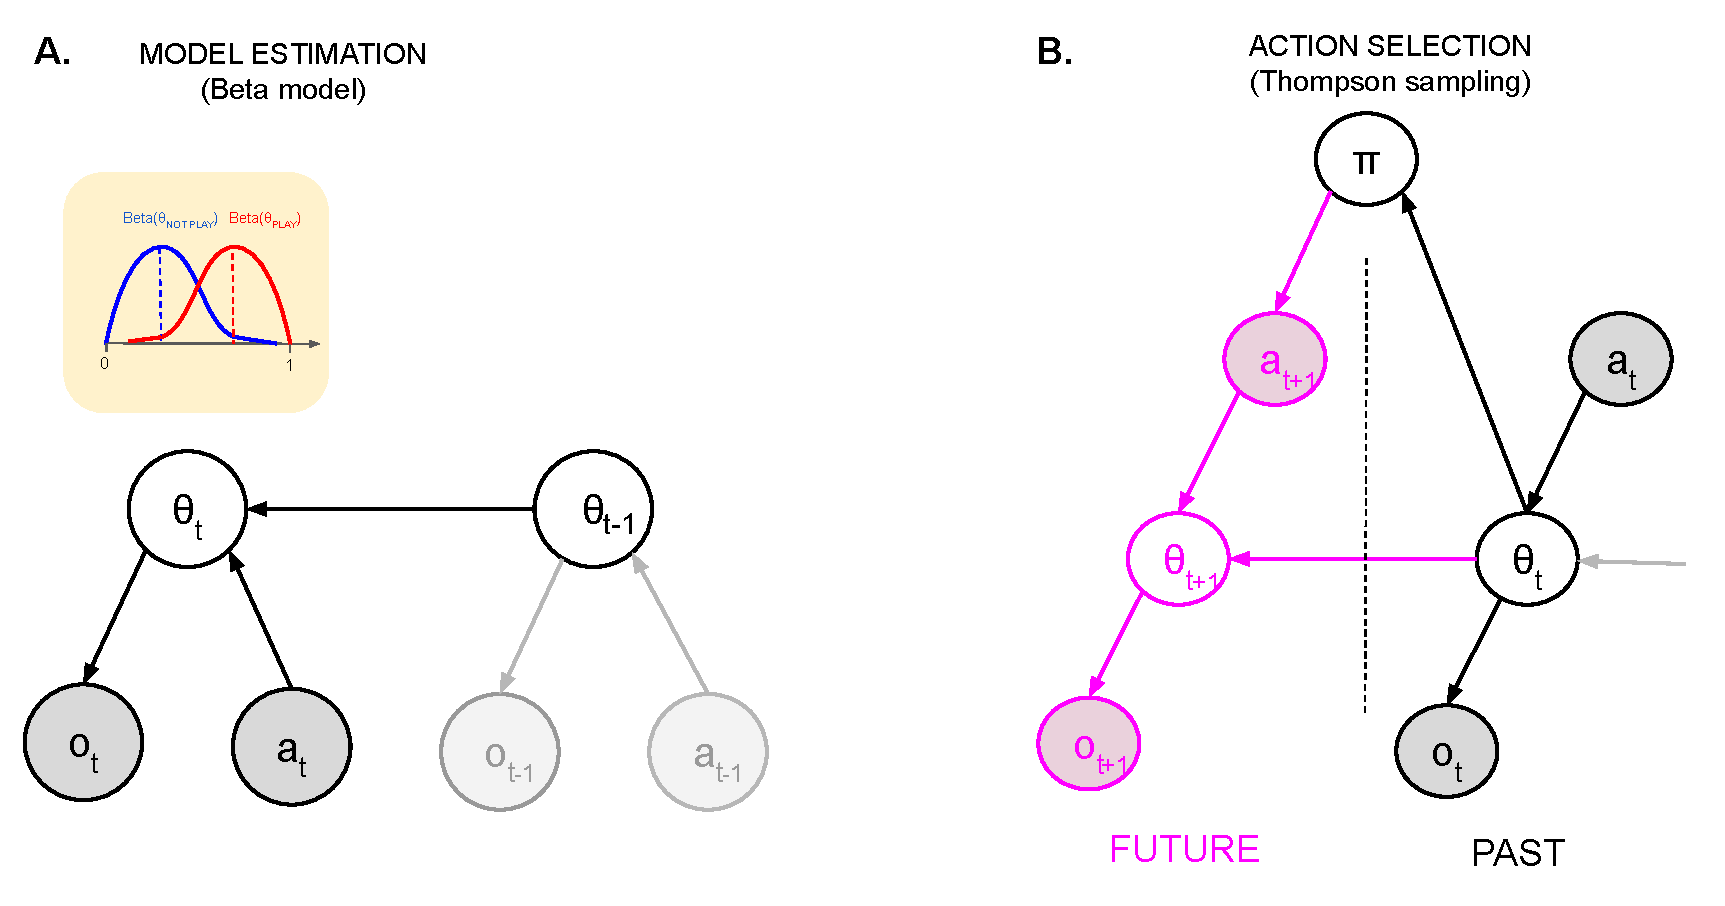
\includegraphics[width=\textwidth]{figs/graphical model.pdf}
\caption{{\bf A. Ideal Observer (parameter estimation)}. Action $a$ and outcome $o$ are the observed variables. A belief on the Bernoulli parameter $\theta$ is inferred from the past estimation and the current observations. {\bf B. Ideal Participant (predictive model of action selection)}. At step $t$, the generative model predicts the next observations from Thompson sampling, allowing to select the next action according to an MLE objective.}
\label{fig:1}
\end{figure}
\subsection{Expected Information Gain (EIG) maximization}



The guiding principle of our ideal participant controller is that actions should serve to sample sensory data.
The objective of the controller is here to provide relevant sensory data to the model, in order to have effective model updates. 
%Many active inference models use objectives that seek to estimate the improvement of the model, relying on a principle of duality \cite{todorov2002optimal}, which states that the action that maximizes the update of the model (learning improvement) is also the one that maximizes the \emph{reduction} of the prediction error.


To do so, we need to formulate the estimation problem under the variational setup that consists in using an upper (or lower) bound of the (negative) prediction error, known as the evidence lower bound (ELBO) [REF] or Variational Free Energy (VFE) [REF]. The data model parameter $\theta$ is considered as a random variable, that obeys to a probability distribution $q_t$, that can evolve during the course of learning, so that $\theta\sim q_t(\Theta)$. 
%In practice, $q_t$ is updated at each time step from observing the data. 
In our case (Bernoulli model), $q_t$ predicts the likely distribution of the Bernoulli parameter of the outcome. After observing the data $o_t$, The observer is considered updating the posterior belief  $q_t$, given $o_t$ and $a_t$, and the previous distribution $q_{t-1}$, %using the chain rule. 
through minimizing the ``Variational Free Energy'' $F(o_t,a_t,q)$:
$$q_t(\Theta|a_t, o_t, h_{t-1}) = \text{argmin}_{q} F(o_t,a_t,q)$$
that is defined as an upper bound on the negative Bayesian evidence (i.e.the ``surprise'')[REF], defined as: %t hat is used to update $q$, defining the optimization after observing $o_t$ and $a_t$:
\begin{align}\label{eq:VFE}
F(o_t,a_t,q) = \mathbb{E}_{\theta\sim q(\Theta)}\left[ -\log p(o_t|\theta) + \log q(\theta) - \log q_{t-1}(\theta)\right]
\end{align}
with  $q_{t-1}(\Theta)$ being the belief about $\theta_t$ before observing the data sample ($a_t$ and $o_t$) and $q(\Theta)$ being the belief about $\theta$ when considering the sample.

The VFE criterion combines the (negative) log-likelihood of the observation under the current model belief with the Kullback-Leibler divergence of the model belief before and after observing the data sample ($a_t$ and $o_t$). The difference between the two distributions, known as the \emph{Bayesian Surprise}, quantifies the reduction of uncertainty provided by observing the data, here:
\begin{align}\label{eq:BS}
\text{KL}(q_t(\Theta)||q_{t-1}(\Theta)) =\mathbb{E}_{\theta \sim q(.|a_t, o_t, h_{t-1})} \log q(\theta|a_t, o_t, h_{t-1}) - \log q(\theta|h_{t-1})    
 \end{align}

This quantity is used in optimization as the regularisation constraint associated with changing the current estimation, that can be interpreted as the ``effort'' needed in the parameter space to reduce the prediction error. 

Interesting to this estimation formula is the role of the free variable $a_t$, i.e. the action. Depending on the choice, it greatly influences the value of the VFE, and more generally exerts a control on the distribution of $\theta$. Put simply, the action conditions the data model of the observation. %, i.e. one can predict what will be observed, given the action. In the context of model estimation and optimization, the action (or the control) plays the role of an auxiliary variable, \emph{allowing to have a control on the observed data}. 
There, the problem become that of minimizing the prediction error under the range of possible controls, knowing that each possible action $a_t$ will conducts to an outcome $o_t$ that can be \emph{predicted} according to the current model. 
This is consistent with the predictive coding principle [REF], interpreted here as \emph{predicting the prediction error}.

{\color{blue} Introducing the expected information gain (EIG)}

Before action selection, one can thus use the generative model to make a prediction about the effect of each action, and choose the one that contributes to minimize the error (or the surprise). 
It becomes obvious however (a well known caveat) that minimizing the prediction error alone, as an ideal observer would do, can not be the objective of the controller, because minimizing the prediction error generally implies minimizing the action diversity (dark room problem, [REF]).
%The problem of action selection in this context proves to be a bit puzzling since the current prediction error does not provide information on which motor decision to make. 
%For convenience, let us consider here $\pi(a_t|h_{t-1})$ the current (implicit) policy and rewrite $q(\theta, a_t|o_t,h_{t-1}) \triangleq q(\theta|a_t,o_t) \pi(a_t|h_{t-1})$. This is the definition of a mixture model that puts $a_t$ in the role of a mixing variable. 
A general solution consists in taking into account duality structure of estimation and control \cite{todorov2001optimal}, that allows to formulate action selection as a min-max problem, that is minimizing the prediction error in the ``worst case'' of action intervention, which gives:

\begin{align}\label{eq:VFE}
\max_{a_t} \mathbb{E}_{\substack{\theta\sim q(\theta|a_t) \\ o_t\sim p(O|\theta)}} \left[\text{min}_{q_t} \mathbb{E}_{\theta\sim q_t(\Theta)} -\log p(o_t|\theta) + \log q_t(\theta) - \log q_{t-1}(\theta)\right]
\end{align}

It is interesting to notice that the Bayesian surprise %here $$\text{KL}(q_{t|t}(\Theta,a_t)||q_{t|t-1}(\Theta,a_t))=\mathbb{E}_{\theta\sim q(.,a_t|o_t,h_{t-1})}\log q(\theta,a_t|o_t,h_{t-1}) - \log q(\theta,a_t|h_{t-1})$$, 
needs here to be \emph{maximized} with respect to $a_t$. It quantifies the amplitude of the expected learning progress, or improved understanding, that should be attained when choosing $a_t$. Put simply, it should conduct to an improved model of the controlled environment.


%Assuming $\theta$ a current statistical model explaining the past observations, we consider here  the process that selects new data in order to feed the model. In principle, one should choose a sample that would reduce the prediction error, i.e. increase the likelihood of the next observations after the model has been updated. 
%reduce the entropy of the posterior, expressed as a KL-divergence between posterior and the prior of the model's belief, a quantity known as the ``Bayesian surprise'' [REF]. Using Bayes formula, it closely corresponds to the . %Incidentally, the expected prediction error itself (before updating the model) is often used as a proxy for future model improvements, explaining the natural attraction toward random/unpredictable outcomes [REF].

  

The Bayesian surprise also writes as an \emph{Information Gain}  $$I(\Theta;a_t,o_t|h_{t-1})=\mathbb{E}_{\theta\sim q(\theta|a_t,o_t,h_{t-1})}\log q(\theta|a_t, o_t, h_{t-1}) - \log q(\theta|h_{t-1}) $$
that is is an estimator of the \emph{mutual information} $I(\Theta;A_t, O_t|h_{t-1})$, quantifying the transmission of information between the data and the model parameters.
At each step, the information gain informs the actor how good the action $a$ is at reducing the uncertainty, that is, in essence, the objective of model learning. %,, that is equal to. In a predictive setup, it is also  
%Here the ``value'' of an observation is reflected in the information it provides to the model. 


\subsection{Information bottleneck in an action/outcome channel}
It is convenient here to remark that the Mutual Information can be decomposed in three terms, i.e. 
\begin{align}\label{eq:MI}
I(\Theta;O_t,A_t|h_{t-1}) &= I(\Theta;O_t|A_t,h_{t-1}) + I(\Theta;A_t|h_{t-1})\\\nonumber
                          &= I(\Theta;O_t|h_{t-1}) + I(\Theta;A_t|h_{t-1}) - I(O_t;A_t|h_{t-1}) 
\end{align}

{\color{gray}
[TO BE VERIFIED]. 

Indeed, it can be remarked here that $I(\Theta;O_t|A_t,h_{t-1})=I(\Theta;O_t|h_{t-1})  - I(O_t;A_t|h_{t-1})$ because 
\begin{align*}
\mathbb{E}_{o_t,\theta, a_t} &\log q(o_t|\theta, a_t, h_{t-1}) - \log q(o_t|a_t, h_{t-1}) \\
                             &= \mathbb{E}_{o_t,\theta, a_t} \log q(o_t|\theta, h_{t-1}) - \log q(o_t|a_t, h_{t-1})\\
                             &= \mathbb{E}_{o_t,\theta, a_t} \log q(o_t|\theta, h_{t-1}) - \log q(\theta|h_{t-1}) + \log q(\theta|h_{t-1}) - \log q(o_t|a_t, h_{t-1})\\
                             &= \mathbb{E}_{o_t,\theta, a_t} \log q(o_t, \theta| h_{t-1}) - \log q(\theta|h_{t-1}) - \log q(o_t|a_t, h_{t-1})\\
                             &= \mathbb{E}_{o_t,\theta, a_t} \log q(\theta|o_t, h_{t-1})  - \log q(\theta|h_{t-1}) + \log q(o_t|h_{t-1}) - \log q(o_t|a_t, h_{t-1})
\end{align*}
}
In that decomposition, it is manifest that $\theta$ plays the role of an intermediary variable that conveys information from $a_t$ toward $o_t$. In information theory, the passing from $a_t$ toward $\theta$ corresponds to an \emph{encoding} while the passing from $\theta$ toward $o_t$ corresponds to a \emph{decoding}. In total, the intermediary variable $\theta$ serves to transmit a message from actions toward observations. It was remarked in \cite{Klyubin2005EmpowermentAU} that maximizing the channel capacity of such an action/outcome setup can serve as a valid objective for action selection, in which case the learning of $q(\theta)$ helps providing an estimate of this capacity. 

The channel capacity considered here is the maximal information that can be passed from $a_t$ toward $o_t$, expressed in bits as :
\begin{align}
\max_{\pi} I_\pi(O_t;A_t) 
= \max_{\pi}\mathbb{E}_{\substack{a_t\sim \pi\\ o_t\sim p(o_t|a_t)}} \log p(o_t|a_t) - \log p(o_t)
\end{align}

An important element of this formula is $\pi$, that is the ``policy'', giving the proportion at which the different actions are chosen over time. It can also be seen as the mixing proportions of a mixture distribution $p(O|\theta,\pi)$. %This proportion was not explicit in our previous formulas, but needs to be considered in the calculation of the channel capacity.

%[role de $\pi$ pour calculer la distribution marginale]

During learning, an approximate channel capacity estimator is provided by the parametric distribution, with {\color{magenta} $I(O_t;A_t)\geq \min(I(\Theta;O_t|h_{t-1}), I(\Theta;A_t|h_{t-1}))$ (A VERIFIER??)}. In particular, $I(\Theta;O_t|h_{t-1})$, is interpreted as the ``information bottleneck'' of the action/outcome channel. Maximising the estimator $\tilde{I}(\Theta;O_t|h_{t-1}) \sim  \log p(o_t|\theta) - \log p(o_t|h_{t-1})$  appears here to be equivalent to maximising the channel capacity of the action-outcome setup, i.e. maximizing the ``Empowerment'' \cite{Klyubin2005EmpowermentAU}.

In practice, at each step $t$ of the estimation process, the empirical $\pi$ gives the proportion at which the different actions are chosen. %From $\pi_t$, one can sample $a_t$ the action at time $t$. 
In our simplified setup, $\pi$ is kept implicit. %, and mostly $a_t$ is chosen (or sampled) during the learning process. %from estimating the maximum bayesian surprise. 
Instead we provide a model of the \emph{effect} of the policy, that is the distribution of outcomes observed so far, resulting from the different actions selected during learning.
This model is called the ``marginal model'' of the outcome, noted $\tilde{p}(o_t) \simeq p(o_t|h_{t-1})$, resulting from the policy adopted so far.

Then, at time $t$, an agent aiming at maximizing the action/outcome channel capacity should consider selecting action maximizing :
\begin{align}
    \max_{a_t} \mathbb{E}_{\theta,o_t\sim q(\theta,o_t|a_t)} \log p(o_t|\theta) - \log \tilde{p}(o_t)
    \label{eq:CC}
\end{align}

The objective being to maximize the channel capacity, one should at each time step choose the action that, in expectation, maximises a non-biased estimator of eq. (\ref{eq:CC}),
where the selection of action should be based on comparing two quantities:
\begin{itemize}
\item The positive term  $\log p(o|\theta)$ reflects a \emph{precision} objective (that is having low prediction errors). This term increases when the value of $\theta$ gets closer to the actual distribution.  
\item while the negative term $ -\log \tilde{p}(o_t) \simeq - \log p(o|h_{t-1}) $ is an estimator of the entropy of the outcome. This term will be kept high if a diversity of outcomes is observed. This sampling diversity objective (state coverage) relies on the marginal model $\tilde{p}$, that should be updated at each step. 
\end{itemize}
Only the combination of both may provide a comprehensive modeling of the environment, that can be attained at the cost of maintaining a general (marginal) model of the observations.   

Importantly, the objective of eq.(\ref{eq:CC}) can be rewritten as $\mathbb{E}_{\theta\sim q(\theta|a_t)} \text{KL} ( p(O_t|\theta)|| \tilde{p}(O_t))$, that is the Kullback-Leibler divergence between the outcome distribution of the current action and that of the marginal distribution. The action that is \emph{the most distant} from the marginal distribution is thus supposed to be selected more often. This "maximum divergence" principle for action selection conducts in fact to an equilibrium state in which both action-outcome distributions should remain at equal distance from the marginal distribution, favouring alternate action selection in the long run. 




%then, considering that the objective of the observer (i.e. the brain) is to develop a good understanding (a good model) of its environment, 


%gives the model consistency while the second one quantifies the model precision.
%Given a current data model (provided by the ideal observer), the ideal participant can estimate how unexpected the outcome is regarding the model, i.e. $-\log p(O|\theta)$, which can be compared to the marginal surprise $-\log p(s)$. The difference $\log p(O|a,\theta) - \log p(O|\theta)$ is the \emph{Information Gain} provided by the action $"a"$.
%Maximizing the information gain turns out, in average,  to
%maximizing the Empowerment \cite{Klyubin2005EmpowermentAU}, which is the channel capacity of an action-outcome medium. The concept is different from that of Bayesian surprise \cite{ITTI20091295}, used in classic (Free Energy based) active inference \cite{friston2012perceptions}.

%\begin{equation}
%    \mathcal{E} = \max_\pi \mathbb{E}_{s\sim \pi(A)} \mathbb{E}_{s\sim p(O|a, \theta)} \log p(O|a,\theta) - \log p(O|\theta, \pi) \label{eq:emp}
%\end{equation}
%This conducts to treat $\log p(O|a,\theta) - \log p(O|\theta,\pi)$ as a reward, 
%which corresponds, for a given data model $\theta$, to choose an action that should maximize the difference between the surprise and the \emph{marginal surprise}, with the marginal distribution of states defined as:
%$$ p(O|\theta,\pi) = \mathbb{E}_{a\sim\pi(a)} p(O|a,\theta)$$

%Idée : l'équation de l'empowerment représente un point d'équilbre entre deux tendances : l'aversion à l'erreur (le modèle doit être précis dans ses prédictions), ce qui revient à minimiser la surprise, mais également une attirance pour la nouveauté, exprimée par le terme d'entropie de la distribution marginale. Cet équilibre entre deux tendances contradictoires   




%As time passes, the belief should converge to a point distribution and the Bayesian surprise should converge to zero.

%This conducts to biasing the selection of action in favour of data that would maximises the update of the model [REF]. However, predicting the information gain is more complex than just predicting the average outcome. 









%It belongs to the family of variational inference algorithms. The model assumes that a . Here the set of parameters $\theta$ take the role of a hidden variable. 

 



%\subsubsection{Approximated active inference for Bernoulli bandit}

% ... (see previous version of the latex document if needed to retrieve info about Active Inference)

\subsection{Learning beyond utility by combining knowledge and behavior improvement}

In everyday life, the pursuit of knowledge (information seeking) often combines with the necessity to achieve certain goals related to survival and social success (reward seeking). The choice of an action or a behavior often involves balancing these two imperatives, a problem often summarized under the term 'exploration/exploitation trade-off'. This problem has been recognized for a long time, but, surprisingly, no consensus formalization seems to have emerged so far.

Indeed, classic learning methodologies often involve the consideration of finite-state models, where the incorporation of the environment's structure (the construction of a model) is only an auxiliary step, generally adressed using ad-hoc heuristics. Indeed, the fact that there is no persistent search for information in machine learning models often relies on the stationary and finite (bounded) nature of most learning problems, a well-known limitation when real-world implementations need to be considered [REF]. Moreover, in engineering, the model is often given in advance, and, in this case, the optimization relies on the inversion of a model (model-based learning) [REF]. In machine learning, optimization often focuses solely on behavioral improvement, based on predefined observation/response patterns (supervised learning), or on an external reward signal, which can be delayed in time (temporal credit assignment problem). Even when the  uncertainty and noisiness of the environment is considered, the target optimal policy is often a deterministic one, aimed at optimizing an average over a noisy (discounted) sum of of rewards.

This is contrary to most observations made in behavioral sciences and ethology \cite{levine2018reinforcement}: humans and animals often tend to maintain an active, and thus random, component in their behavior, even in the presence of problems with an optimal solution. The presence of an exploration component cannot be explained in terms of optimal control and must therefore be addressed within a framework that considers the gain of information as an objective in itself, not subordinated to the maximization of rewards.

{\color{blue} Nevertheless, and this is the point we are developing here, there can be a truly relevant aspect to maintaining an information term, in the sense that the knowledge one can have of a model can grow almost indefinitely, far beyond the utility it provides. }

Combining information and reward maximization in a same optimization procedure can be solved in a relatively simple manner once considering behavior improvement as a part of knowledge improvement. In short, a same formalisation can be applied to the learning of the parameters of a policy and to the ones utilized in the learning of the model. Here we consider the case where  a single policy is used both for knowledge improvement and behavior improvement.

Then, improving the behavior implies fitting an empirical policy to the observed extrinsic rewards, in a fashion very similar to the one proposed in \cite{haarnoja2018soft}.
In our problem at hand, a statistics over action selections can be provided from observing choices over time. This is the case, for instance, for a coach that would select (or not) a player for matches. Assume now that $\phi=(\pi, \theta)$ with $\pi$ a parameter for action selection (reflecting a proportion of action, i.e. ``PLAY'' or ``NOT PLAY'') and $\theta$ a parameter for predicting the outcome (i.e. ``WIN'' or ``LOSE''). Here $\pi$ would reflect the choices of the coach, and $q(\PI)$ (action selection statistics) could be updated at each step. %Knowing $\theta_x$ would help to provide a more comprehensive model of the way the observations are generated. 
%\text{max}_{x_t}\text{KL}(q_{t|t}(\Pi, \Theta)||q_{t|t-1}(\Pi, \Theta))
%\end{align}
Then, each observation of $o_t$, knowing $a_t$, would allow to improve the generative model by: \begin{align}\label{eq:BS-joint}
I(\Theta,\Pi;a_t,o_t|h_{t-1})= \mathbb{E}_{\theta,\pi\sim q(\theta,\pi|a_t,o_t,h_{t-1})}\log q(\theta,\pi|a_t, o_t, h_{t-1}) - \log q(\theta,\pi|h_{t-1}) 
\end{align}
reflecting both the knowledge improvement about the coach's behavior and match's outcome after observing the data sample.


Importantly here,  an additional element (reward information) comes into the play. In effect,  $o_t$ also indicates whether the choice was correct or incorrect (``WIN'' or ``LOSE''). %In a RL setup, this can be interpreted as an incentive to bias the coach's choice (i.e $\theta_x$) in favor of a policy parameter that would increase the probability of winning. 
Consider for instance $\theta$ being the ``WIN'' expectation of a Bernoulli distribution. Assuming $\pi$ being the ``PLAY'' expectation, then taking $\pi \propto\exp(\theta)$ would be consistent with biasing the selection of action toward maximizing the ``WIN'' expectation [ref Levine]. More generally, %assuming such strategy should be adopted by the coach, 
this correspondence may be given by $q(\Pi|a_t, o_t, h_{t-1})$, i.e. a belief about $\pi$ (action selection) given the outcome (i.e. the action validity), and, more generally, the history of previously observed actions and outcomes. Injecting this relation into equation (\ref{eq:BS-joint}) may thus allows to incorporate reward information into the information gain maximization. This would conduct to a concurrent (or dual) optimization, reflecting both knowledge and action validity improvement (see also \cite{dauce2022concurrent}).

A possible relation between a information gain on the parameters of a behavior model and the maximization of rewards is given by the policy matching approach, originally proposed by \cite{haarnoja2018soft}, where the parameters of a policy $\pi(a)$ are matched to the reward expectation.
The inclusion of the entropy term in the optimization formulation relies on a temperature parameter, analogous to what can be found in stochastic optimization algorithms. This parameter, denoted as $\beta$ (inverse temperature), is involved in the actor's optimization formula as follows:
$$\max_\pi \mathbb{E}_{a\sim \pi(a)} \left(\log p^*(a|Q) - \log \pi(a)\right) = \max \left(\beta Q(a) - \log \pi(a)\right)$$
Here, $Q(a)$ represents the action value function (the critic), and $\pi(a)$ represents the policy (or actor), viewed as a probability distribution over actions. Interpreted in our informational setup, action selection appears to rely on maximizing an information gain between the value parameters of the value and the action.  

Adapted to our mixed information gain setup, the policy matching naturally combines in two expected information gains (EIG) like :
\begin{small}
\begin{align}\label{eq:BS-SAC}
\max_{a_t} \mathbb{E}_{o_t} \mathbb{E}_{\substack{\pi \sim q(\pi|a_t,h_{t-1})\\ \theta\sim q(\theta|a_t,o_t,h_{t-1})}} \left[\log q(\theta|a_t, o_t, h_{t-1}) - \log q(\theta|h_{t-1})\right] + \left[\log q^*(\pi|a_t, o_t, h_{t-1}, \beta) - \log q(\pi|h_{t-1})\right]
\end{align}
\end{small}
with $q^*$ a target distribution on the policy parameters estimated from the current action, outcome and history, and $\beta$ the inverse temperature. Notably, the right EIG term can be connected to the policy matching from Bayes inversion (see Appendix [TODO]). It is important to notice the strong formal similarity between the two EIG terms, implying in both case to compare a KL divergence between a ``data informed'' posterior distribution and a ``marginal'' prior distribution of the parameters. An important difference though is that $\theta$ is sampled from the posterior (i.e. knowing $a_t$ and $o_t$), while $\pi$ is sampled from the prior only, with the parameters of the ``marginal''  policy. The consequence is that the first term corresponds to a maximization of the divergence, while the second implements a minimization (minimizing a divergence between the policy and exponentiated rewards). Each term defines a distinct objective (maximizing information vs. matching the behavior to the rewards), which naturally conducts to find a compromise, i.e. effectively implements a trade-off between exploration and exploitation (see also \cite{dauce2022concurrent}).


%Then assuming $q_{t|t-1}(\Pi)$ the current belief (obtained from observing the coach's choices), one should consider maximizing:
%\begin{align}\label{eq:BS-cond}\text{max}_{x_t}\text{KL}(q_{t|t}(\Pi|\Theta)||q_{t|t-1}(\Pi)) 
%\end{align}
%the information gain about the behavior, reflecting the (expected) behavior improvement expected from considering outcomes. 

%The complementary conditional distribution is $q(\Theta|Q)$ (a belief about $\theta$ given a belief about $Q$).
%In a predictive setup, one can now predict the next update of $\Theta$ knowing the current belief on $Q$. This is noted $q_t(\Theta,Q) = q_t(\Theta|Q)q(Q) $ = a winning probability, then one can assume . Assuming 
%$$\text{KL}(q_{t}(Q|\Theta)||q_{t-1}(Q)) + \text{KL}(q_{t}(\Theta)||q_{t-1}(\Theta|Q))$$
%reflecting the separation of the optimization in two terms. The left one reflecting the update of $Q$ after observing $x_t$ and $y_t$, and the right being the data model improvement, knowing $Q$.

%The information gain can be rewritten as: 
%with the left term reflecting the ``matching'' of the coach's choice with the proportion of ``WIN'', and more generally the matching of the behavior with rewards. The putative mismatch between $Q$ and $\Theta$ development of the formula, given in the algorithm, conducts to 

\subsection{Information seeking Thompson sampling and the ideal participant}
%Inspired by the Bayesian ideal observer \cite{geisler1989sequential}, 
We  develop a model of optimal sampling that we call the ``ideal participant''. An ideal participant is defined as an action selection mechanism (an "actor") that is built on top of an ideal observer.
%Let ${D}_{t}=(a_1,o_1), ..., (a_t,o_t)$ be a sequence of observations; a Bayesian observer is a recursive parameter update strategy that relies on Bayes formula, i.e. $q(\theta|\mathcal{D}_n) \propto p(o_n|a_n, \theta) \times q(\theta|\mathcal{D}_{n-1})$. An important element is the initial \emph{prior} $q_0(\theta)$ reflecting the initial guess about the parameters. 
%In an active sampling strategy, one need to consider specific series of actions $(a_1,...,a_n,...)$, and estimate how the corresponding  observations participates in reducing the uncertainty of the observer. 
If the role of the observer was to build a  model $\theta$, reflecting the statistics of the outcomes, %obtained under any action $a$, 
the role of the agent (ideal participant) is to choose the next action.

A classic (naive) viewpoint on model estimation is that the agent should move freely (randomly) in order to allow the estimation process to identify environment states, and use the model to improve its behavior once enough evidence has been collected from the environment. %, that ultimately may help the controller take good decisions. The two problems (estimating the model and control) are generally considered as independent. Moving freely (independently if the model) may indeed be a god strategy   
Nevertheless, many situations prevent exhaustive (uniform) sampling of the environment before making a decision, particularly in cases where data access is costly or the number of actions is limited. The question then arises as to which action to choose in order to produce the best model in a limited time/resources.

In our model-based setup, instead of calculating the expectation, we rather consider doing \emph{prediction by sampling}, that means considering the result of sampling the generative model associated with each action $q(\theta,s|a)$, consistently with the Thompson sampling principle [REF].  
In our Bernoulli case,  each action is associated with a Beta model, and estimating the channel capacity consists for each action $a$ in:
\begin{itemize}
    \item (i) sampling the Bernoulli parameter $\tilde{\theta}_a$ from the Beta model,
    \item (ii) sampling the Bernoulli parameter $\tilde{\theta}$ from the marginal model
    %\item (ii) generating an outcome $\tilde{o}_a$ by sampling the Bernoulli model,
    %\item (iii) calculating the log-probability difference : $\log p(\tilde{o}_a|\tilde{\theta}_a) - \log \tilde{p}(\tilde{o}_a)$
    \item (iii) estimating $\text{KL}(p(O|\tilde{\theta}_a)||p(O|\tilde{\theta})|)$
\end{itemize}   
and select the action with maximum value. 

This selection of action $a_t$ (action sampling) is then followed by:
\begin{itemize}
\item (iv) observing the outcome $o_t$
\item (v) updating the Beta model $q(\Theta|a_t)$
\item (vi) updating the marginal model $\tilde{q}(\Theta)$
\end{itemize}


\subsection{Biased participants}




\section{Experiments}


\section{Results}
%Ideal observer models  are used to estimate, in perception tasks, how subjects deviate from an optimal response, knowing the parameters of a task. 
We are interested here in the action selection strategies developed by the subjects, and by the action selection \emph{biases}. In such a setup it is easy to show that a close to optimal strategy is to choose the actions 'PLAY' and 'NOT PLAY' in equal proportion. A first and important observation is that human subjects exhibit mostly irregular action selection, resembling that of a Bernoulli draw, rather than a periodic alternation. %A second observation is that they manifest significant biases toward the actions that provide higher rewards (that is the "reward bias"), which reflects a compelling preference to 'WIN' rather than 'LOSE', which is largely expected in this kind of setup (not shown). 

More intriguingly, a significant bias toward entropic (action, outcome) relationships is observed in experiment A only (that is action-outcome relationships that are "difficult" to predict). In order to quantify this entropy bias, the entropy difference $\Delta H = H(p_1) - H(p_0)$, where $H(p)=-\sum_{s \in S}p(s)\log(p(s))$ is the entropy, indicates whether $p_1$ is more (or less) irregular than $p_0$. %The entropy difference bias can be seen as resulting from an imbalance between the precision and the diversity objectives, 
The question comes why such an imbalance is observed in the first experiment and not in the second? We thus simulated an ``ideal participant'' resolving similar tasks.
The ideal observer builds a posterior $q(\theta) = (\beta(n_{\text{WIN}}^{\text{PLAY}}, n_{\text{LOSE}}^{\text{PLAY}}), \beta(n_{\text{WIN}}^{\text{NOT PLAY}}, n_{\text{LOSE}}^{\text{NOT PLAY}}))$, with $\beta$ a beta model with $n_s^a$ being the number of $(a,s)$ observations. The marginal distribution $\beta(n_{\text{WIN}},n_{\text{LOSE}})$ is estimated in addition.
Then, the ideal participant samples $ \tilde{p}_0,  \tilde{p}_1$ from the ideal observer, estimates the marginal $\tilde{p}_\text{m}$, and the action chosen is the one that maximizes the Kullback-Leibler divergence $KL(\tilde{p}_i||\tilde{p}_\text{m})$, with $i$ in $\{0,1\}$.
The differences between experiment A and experiment B are implemented in the \emph{priors} of the ideal observer (see figure \ref{fig:data}), that is the prior of $p_0$, $p_1$ and $p_m$ based on the experiment design. In experiment A, those distributions are identically distributed over the [0.2,0.8] range, while in experiment B, the prior distribution of $p_0$ is skewed to the left, while the prior distribution of $p_1$ is skewed to the right. This single difference has for consequence that the prior of $p_0$ and $p_1$ is less informative in experiment A than in experiment B. This uninformative prior implies a longer training in experiment A than in experiment B, which conducts to place a greater emphasis on the diversity objective. As a result, action selection in experiment A tended towards highly entropic outcomes.

\begin{figure}[t!]
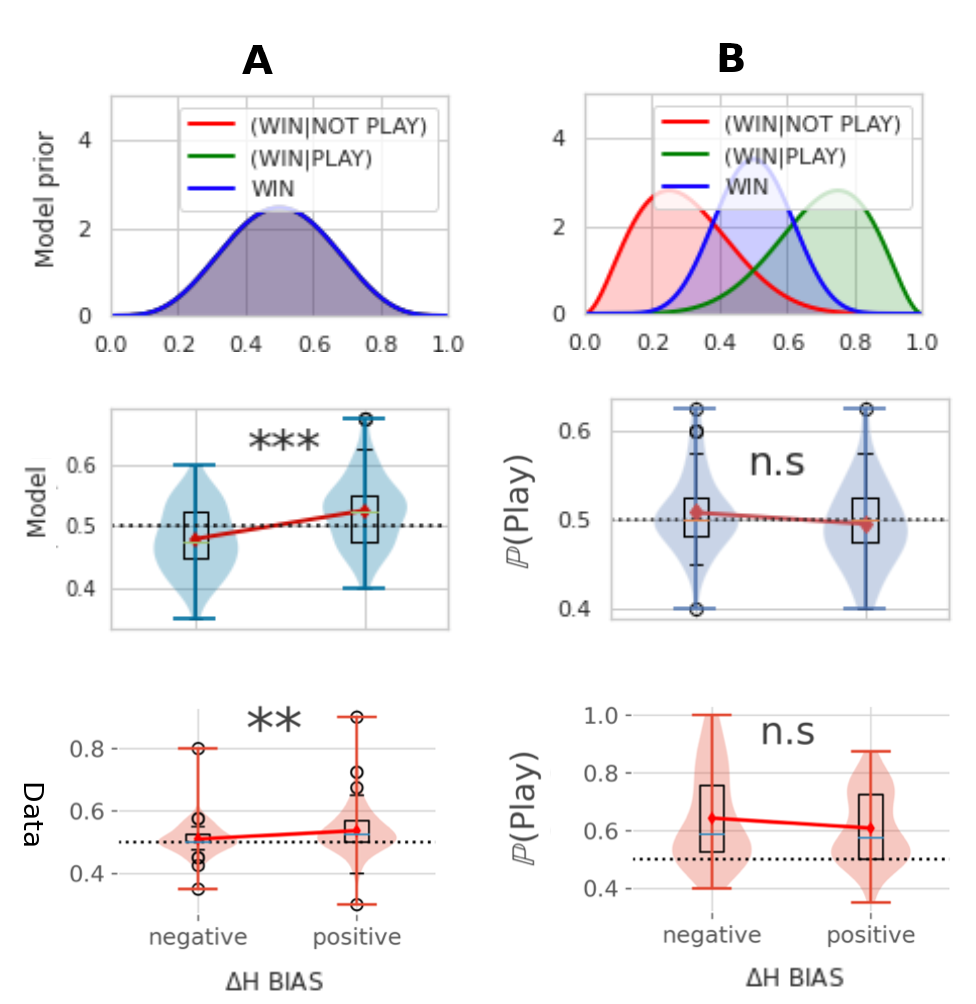
\includegraphics[width=.8\linewidth]{figs/cosyne_analysis.png}

\caption{{Action selection biases in models and experiments}. Left column : Experiment A (both positive and negative contingencies). Right column : Experiment B (only positive contingencies). Top row: the prior given to the observer in the two different setups. 
%MEG data (left) where participant were healthy and the task had negative causality values. SEEG data (right) from epileptic patients who had an easier task with only positive causality values. 
%The model'prior represent the difference between the setups of SEEG and MEG data. (B) 
Second row : The ratio of the action "PLAY" generated by the ideal participant, given the prior and the value of $\Delta H$. The difference is significant in Experiment A (left, $p<0.001$). %It means the model selects the action 'Play' when it is more entropic i.e its outcome is more random. 
This is not the case in Experiment B (right, $p>0.05$). Third row: behavioral data collected from participants. (Left) Participants show a significant bias toward more surprising actions (left, $p<0.01$).  (right) No significant difference in action selection. These findings match those of the model.
}
\label{fig:data}
\end{figure}

% This action selection relies on a tight balance between two opposing tendencies, namely (ii) making correct predictions, and (ii) providing sufficiently diverse data to feed the models. 
%An important confounding factor, however, is that Experiment A was conducted with healthy subjects while Experiment B was conducted with epileptic patients, although the behavioral responses were consistent in both types of subjects. 

These results finally confirm our assumptions, suggesting that human subjects may develop information-guided action selection strategies, by combining principles of Bayesian estimation \cite{knill2004bayesian} and action read-out information maximization \cite{Klyubin2005EmpowermentAU}. Furthermore, ongoing research is underway in the laboratory to investigate whether such action-selection principles can be detected in electrophysiological signals.


\section*{Acknowledgments}
Cras egestas velit mauris, eu mollis turpis pellentesque sit amet. Interdum et malesuada fames ac ante ipsum primis in faucibus. Nam id pretium nisi. Sed ac quam id nisi malesuada congue. Sed interdum aliquet augue, at pellentesque quam rhoncus vitae.

\section*{Supporting information}

\subsection{Note on action selection metrics (2022)}

We build a \emph{model} of an agent having to take decisions in a stochastic environment where the result of the action (outcome) is uncertain.
We assume that the agent has to learn the effect of its action by interacting with the environment. During learning, the agent builds a statistical model of its environment but also updates its \emph{policy} (selection of actions). Both the model and the policy are parametric models. 

Notations :
\begin{itemize}
    \item $a \in \mathcal{A}$ : action (decision or motor command)
    \item $s \in \mathcal{S}$ : state observed after action $a$ is actuated
    \item $r \in \mathbb{R}$ : (quantitative) reward 
    \item $Q(a)$ : action-value function = policy parameters
    \item $\pi(a|Q)$ : (stochastic) action selection = policy
    \item $\theta$ : model parameters (mean, variance)
    \item $p(s|a, \theta)$ : parametric model of state transitions
    \item $q(\theta)$ : (posterior) distribution of model parameters. In practice : $\beta$-model 
\end{itemize}

Classically, the model parameters $\theta$ and the policy parameters $Q$ are trained independently. 
Let $\mathcal{D}_n = (a_1, s_1, r_1), ..., (a_n, s_n, r_n)$ be a sequence of (action, state and outcome) triplets.
Both models are trained online.
For instance, the action-value is classically updated using a reward prediction error : 
\begin{align}
     \text{RPE}_n &= r_n - Q_{n-1}(a_n)\nonumber\\
     Q_n(a_n) &= Q_{n-1}(a_n) + \eta \text{RPE}_n\nonumber
\end{align}
with $\eta$ a learning parameter, and
$$q(\theta|\mathcal{D}_n) \propto p(s_n|a_n, \theta) \times q(\theta|\mathcal{D}_{n-1})$$
(Bayes rule and ideal observer).

This conducts to a classic exploration/exploitation dilemma. The data that is sampled depends on the policy and the classic reinforcement learning policies tend to over-sample the rewarding states and sub-sample the non-rewarding or punishing state.  For instance, the use of a softmax stochastic policy $\pi(a) \propto \exp(Q(a))$ provides a state imbalance in favor of the more rewarding actions and this action imbalance renders the model less accurate.

The causal project addresses the question of action selection when the main objective is to learn a model of the action-outcome relationship, in order to make an appropriate ``buy'' decision. In that case, the participant need to find a policy that optimizes a different objective, that is understanding the setup and correctly estimate the model.

In vision, the saliency metric was proposed by Itti and Baldi \cite{itti2009bayesian}, to report the fact that the eye is attracted by the part of a visual scene that is the most surprising regarding the data model.
Let $\theta$ be the parameters of the visual model, and $a$ be the direction of sight, then the ``value'' of $a$ is $$\text{KL}(q(\theta|a)||q(\theta))$$ that is called the salience (or Bayesian surprise). The salience is maximal when the divergence is maximal.

Taking inspiration from Itti and Baldi, the idea here is to use a policy that should maximize the knowledge about the data model. That is the policy that maximizes the divergence :
$$\text{KL}(q(\theta|\pi)||q(\theta))$$
In short, this means  finding a policy that provides more sample efficient data to the model than any random policy.

In a sequential approach, we need to consider the improvement of a current policy $\pi_{n-1}$, given a data model $q_{n-1}$, that is :
$$\pi_n = \max_{\pi}\text{KL}(q_n(\theta|\pi)||q_n(\theta|\pi_{n-1}))$$
In detail, a saliency-optimal policy that reduces the entropy of $q_n(\theta)$, knowing the current policy $\pi_{n-1}$, and $q_{n-1}$ the current data model, is:
\begin{align}
&\max_a \text{KL}(q_n(\theta|a, \pi_{n-1})||q_n(\theta|\pi_{n-1}))\nonumber\\
\sim &\max_a \log p(s|a,\theta) q_{n-1}(\theta) - \log \mathbb{E}_{a'\sim\pi_{n-1}(a)} p(s|a',\theta) q_{n-1}(\theta)\nonumber\\
= &\max_a \log p(s|a,\theta) - \log p(s|\theta, \pi_{n-1})\nonumber
\end{align}
This conducts to treat $\log p(s|a,\theta) - \log p(s|\theta)$ as a reward, which corresponds, for a given data model $\theta$, to choose an action that should maximize the difference between the surprise and the \emph{marginal surprise}, with the marginal surprise defined as:
$$ p(s|\theta,\pi) = \mathbb{E}_{a\sim\pi(a)} p(s|a,\theta)$$

Interestingly, this is consistent with maximizing a well-known action selection metric called the empowerment \cite{klyubin2005empowerment}.  The empowerment is defined as the maximal channel capacity in an action-outcome setup, which corresponds to maximizing the mutual information between the action and the outcome. 
$$\mathcal{E} = \max_\pi \mathbb{E}_{s,a\sim p(s,a|\theta,\pi)} \log p(s|a,\theta) - \log p(s|\theta, \pi)$$


\subsection*{Combining reward and information gain objectives}
{\color{blue}


[WORK IN PROGRESS]




On contrary to an observer, a reinforcement learning algorithm exerts a \emph{control} on the data it collects. Like in Thompson sampling, the observer may thus be an element of a larger estimation process that would take action over and causal relations within the data into consideration. 

Though generally assumed to maximize the reward expectation, the sampling of the data remains an important part of the process. It has been the subject of an abundant literature in the RL and robotics community, in order to go beyond the baseline uniform sampling on actions ($\varepsilon$-greedy). This comprise different variants of novelty detection, learning improvement and curiosity metrics [REFS]. Such exploration-incentive metrics remain however quite arbitrary and ``hand-made'', and remain difficult to incorporate into the RL optimization framework. 


Additionally, one can also provide a statistics over action selections from observing choices over time. This is the case, for instance, for a coach that would select (or not) a player for matches. Assume now that $\phi=(\pi, \theta)$ with $\pi$ a parameter for action selection (reflecting a proportion of action, i.e. ``PLAY'' or ``NOT PLAY'') and $\theta$ a parameter for predicting the outcome (i.e. ``WIN'' or ``LOSE''). Here $\pi$ would reflect the choices of the coach, and $q(\PI)$ (action selection statistics) could be updated at each step. %Knowing $\theta_x$ would help to provide a more comprehensive model of the way the observations are generated. 
Then, each observation of $y_t$, knowing $x_t$, would allow to improve the generative model by: \begin{align}\label{eq:BS-joint}
\text{max}_{x_t}\text{KL}(q_{t|t}(\Pi, \Theta)||q_{t|t-1}(\Pi, \Theta))
\end{align}
reflecting both the knowledge improvement about the coach's  behavior and match's outcome after observing the data sample.

Importantly here,  an additional element (reward information) comes into the play. In our case,  $y_t$ would indicate whether the choice was correct or incorrect (``WIN'' or ``LOSE''). %In a RL setup, this can be interpreted as an incentive to bias the coach's choice (i.e $\theta_x$) in favor of a policy parameter that would increase the probability of winning. 
Consider for instance $\theta$ being the ``WIN'' expectation of a Bernoulli distribution. Assuming $\pi$ being the ``PLAY'' expectation, then taking $\pi \propto\exp(\theta)$ would be consistent with biasing the selection of action toward maximizing the ``WIN'' expectation [ref Levine]. More generally, %assuming such strategy should be adopted by the coach, 
this correspondence may be given by $q(\Pi|\Theta)$, i.e. a belief about $\pi$ (action selection) given the belief about $\theta$ (the outcome i.e. the action validity). Injecting this relation into equation (\ref{eq:BS-joint}) may thus allows to incorporate reward information into the information gain maximization. This would conduct to a concurrent (or dual) optimization, reflecting both knowledge and action validity improvement (see also \cite{dauce2022concurrent}).
%Then assuming $q_{t|t-1}(\Pi)$ the current belief (obtained from observing the coach's choices), one should consider maximizing:
%\begin{align}\label{eq:BS-cond}\text{max}_{x_t}\text{KL}(q_{t|t}(\Pi|\Theta)||q_{t|t-1}(\Pi)) 
%\end{align}
%the information gain about the behavior, reflecting the (expected) behavior improvement expected from considering outcomes. 

%The complementary conditional distribution is $q(\Theta|Q)$ (a belief about $\theta$ given a belief about $Q$).
%In a predictive setup, one can now predict the next update of $\Theta$ knowing the current belief on $Q$. This is noted $q_t(\Theta,Q) = q_t(\Theta|Q)q(Q) $ = a winning probability, then one can assume . Assuming 
%$$\text{KL}(q_{t}(Q|\Theta)||q_{t-1}(Q)) + \text{KL}(q_{t}(\Theta)||q_{t-1}(\Theta|Q))$$
%reflecting the separation of the optimization in two terms. The left one reflecting the update of $Q$ after observing $x_t$ and $y_t$, and the right being the data model improvement, knowing $Q$.

%The information gain can be rewritten as: 
%with the left term reflecting the ``matching'' of the coach's choice with the proportion of ``WIN'', and more generally the matching of the behavior with rewards. The putative mismatch between $Q$ and $\Theta$ development of the formula, given in the algorithm, conducts to 


} 



\nolinenumbers

% Either type in your references using
% \begin{thebibliography}{}
% \bibitem{}
% Text
% \end{thebibliography}
%
% or
%
% Compile your BiBTeX database using our plos2015.bst
% style file and paste the contents of your .bbl file
% here. See http://journals.plos.org/plosone/s/latex for 
% step-by-step instructions.
% 

%\begin{thebibliography}{10}

%\bibitem{bib1}
%Conant GC, Wolfe KH.
%\newblock {{T}urning a hobby into a job: how duplicated genes find new
%  functions}.
%\newblock Nat Rev Genet. 2008 Dec;9(12):938--950.

%\bibitem{bib2}
%Ohno S.
%\newblock Evolution by gene duplication.
%\newblock London: George Alien \& Unwin Ltd. Berlin, Heidelberg and New York:
%  Springer-Verlag.; 1970.

%\bibitem{bib3}
%Magwire MM, Bayer F, Webster CL, Cao C, Jiggins FM.
%\newblock {{S}uccessive increases in the resistance of {D}rosophila to viral
%  infection through a transposon insertion followed by a {D}uplication}.
%\newblock PLoS Genet. 2011 Oct;7(10):e1002337.

%\end{thebibliography}

\bibliographystyle{apalike} 
%\setlength{\bibleftmargin}{.125in}
%\setlength{\bibindent}{-\bibleftmargin}

\bibliography{biblio}
%\printbibliography

\end{document}



